\documentclass[aspectratio=169,11pt]{ctexbeamer}

\usetheme{Madrid}
\usecolortheme{default}
\setbeamertemplate{navigation symbols}{}
\setbeamertemplate{footline}[frame number]
\setbeamertemplate{itemize item}{\small\raise1.2pt\hbox{$\blacktriangleright$}}
\setbeamertemplate{itemize subitem}{\tiny\raise1.2pt\hbox{$\bullet$}}

\usepackage{amsmath,amssymb,mathrsfs,booktabs,array,multirow}
\usepackage{graphicx}
\usepackage{tikz}
\usetikzlibrary{arrows.meta,positioning,fit,shapes.misc,backgrounds}
\usepackage{xcolor}
\usepackage{ragged2e}

\let\solution\relax
% ========== Sets ==========

% Planning horizon start
\newcommand{\planningStart}{\alpha}

% Planning horizon end
\newcommand{\planningEnd}{\beta}

% Time discretization step
\newcommand{\discretizationStep}{\Delta}

% Airport-specific initial discretization step (travel-time based)
\newcommand{\initStep}{s} % _{i}

% Check time
\newcommand{\checkTime}{t_c}

% Time discretization set
\newcommand{\discretization}{\mathcal{T}}

% Full time discretization set
\newcommand{\discretizationFull}{\hat{\discretization}}

%  ----------------- Network -------------------

% Flat Network $\netFlat=(\airportSet, \segSet)$
\newcommand{\netFlat}{\mathscr{G}}

% Set of airports
\newcommand{\airportSet}{\mathcal{I}}

% Set of segments indexed by $s$
\newcommand{\segSet}{\mathcal{S}}

% Distance for segment s
\newcommand{\distance}{D} % _{s}

% Time-Expanded Network $\net{\discretization}=(\nodeSet, \arcSet)$
\newcommand{\net}{\mathcal{G}} % {\discretization}

% Required frequency for segment s
\newcommand{\freq}{n} % _{s}

% Travel time for segment
\newcommand{\travelTime}{\tau} % _{s}

% Minimum interdeparture time
\newcommand{\minInterdepTime}{g} % _{s}

% Set of nodes
\newcommand{\nodeSet}{\mathcal{N}}

% Set of arcs
\newcommand{\arcSet}{\mathcal{A}}

% Flight arcs set notation
\newcommand{\flightArc}[1][{}]{{\arcSet^F_{#1}}}

% Departure arcs set notation
\newcommand{\departArc}{{\mathcal{D}}}

% Holding arcs set notation
\newcommand{\holdingArc}[1][{}]{{\arcSet^H_{#1}}}

% Holding incoming arcs
\newcommand{\holdingArcIn}{\mathcal{H}_{in}}

% Holding outcoming arcs
\newcommand{\holdingArcOut}{\mathcal{H}_{out}}

% Impossible departure numbers
\newcommand{\impDeparts}{Q}

% Red-eye arcs set notation
\newcommand{\redArc}{{\arcSet^R}}

% Serving arcs set notation
\newcommand{\servingArc}{{\arcSet^{S}}}

% Positioning arcs set notation
\newcommand{\positionArc}{{\arcSet^{P}}}

% Set of outgoing arcs from node (i,t)
\newcommand{\outArcSet}[1]{{\arcSet^{+}_{#1}}} % {i,t}

% Set of incoming arcs to node (i,t)
\newcommand{\inArcSet}[1]{{\arcSet^{-}_{#1}}} % {i,t}

% Set of flight arcs from node (i, $\cdot$) and fleet type is $f$
\newcommand{\outArcSetByF}[1]{{\arcSet^{+}_{#1}}} % {i,f}

% Set of flight arcs to node (i, $\cdot$) and fleet type is $f$
\newcommand{\inArcSetByF}[1]{{\arcSet^{-}_{#1}}} % {i,f}

% Set of holding arcs at time tc
\newcommand{\holdingArcTc}[1]{{\arcSet^H(#1)}} % {t_c}

% Set of flight arcs at time tc
\newcommand{\flightArcTc}[1]{{\arcSet^F(#1)}} % {t_c}

% Set of invert arcs at time tc
\newcommand{\invertArcTc}[1]{\overleftarrow{\arcSet}(#1)} % {t_c}

% Set of arcs for segment s at time t
\newcommand{\arcDuringSepTime}{D} % _{ijt}

% Aggregated departure flow in a separation window for segment (i,j) starting at t
\newcommand{\arcDepartFlow}{F^{\text{dep}}} % _{ijt}

% Number of flights which can depart in the interval $[t, t+\minInterdepTime_{ij})$
\newcommand{\departLimit}{\xi} % _{ijt}

% Combined Limit
\newcommand{\combLimit}{\bar{\xi}} % _{R}

% Set of arcs for segment s
\newcommand{\segArcSet}[1]{\arcSet(#1)} % {s}

% Segment of arc a
\newcommand{\sfa}[1]{s({#1})} % {a}

% Separation Violation Amount
\newcommand{\sepViolAmount}{V^{\text{sep}}} % _{ij}(t)

% Separation Violation Flow
\newcommand{\sepViolFlow}{N} % _{ijt}

% summation of the separation violation amount $\sepViolAmount_{ijt}$ and the illegal departure quantities $\impDeparts(i,t,f)$ and $\impDeparts(j,t,f)$
\newcommand{\sepInterViolAmount}{\mathscr{V}} % _{ijt}

% Cumulative Departures
\newcommand{\cumDepart}{D} % _{jf}(t)

% Cumulative Real Arrivals
\newcommand{\cumArrReal}{A^{\text{real}}} % _{jf}(t)

% Late Arrival Set
\newcommand{\lateArrSet}{\mathcal{A}_{\text{late}}}

% Discreted Path Signature of itinerary r
\newcommand{\pathSig}[1]{\pi({#1})} % {r}

% Equivalence class of itineraries by discreted path signature
\newcommand{\eqClassByPathSig}{S} % _{(R)}

% Equivalence relation by discreted path signature
\newcommand{\eqRelByPathSig}{\sim}

% Original Path of itinerary r
\newcommand{\origPath}[1]{\hat{\pi}({#1})} % {r}

% Equivalence class of itineraries by original path signature
\newcommand{\eqClassByOrigPath}{\mathscr{O}} % _{r'}^{r}

% Equivalence relation by original path signature
\newcommand{\eqRelByOrigPath}{\hat{\sim}}

% Itinerary Combination Set
\newcommand{\itinCombSet}{\mathscr{I}}

% Compatible Combination Set for super-itinerary R (optional method index)
\newcommand{\compatSet}[2][]{\mathcal{C}^{#1}(#2)} % [method]{R}

% Max Attraction Combination Set
\newcommand{\maxAttrCombSet}{\itinCombSet^{*}} % _{rp\ell}

%  ----------------- Market -------------------

% Set of markets
\newcommand{\marketSet}{\mathcal{M}}

% Set of passenger types
\newcommand{\psgTypeSet}{\mathcal{P}}

% Set of fare classes
\newcommand{\fareClassSet}{\mathcal{L}}

% Set of itineraries
\newcommand{\itinSet}{\mathcal{R}}

% Set of super-itineraries
\newcommand{\itinSetSuper}{\itinSet^{*}}

% Set of remaining super-itineraries
\newcommand{\remainingItienSetSuper}{\bar{\itinSetSuper}}

% Set of itineraries in market m
\newcommand{\itinInMarket}{R} % _{m}

% Set of super-itineraries in market m
\newcommand{\itinSuperInMarket}{R^{*}} % _{m}

% Set of itineraries in market m that use arc a
\newcommand{\itinUsingArc}[2]{R_{#1}(#2)} % {m}{a}

% Set of super-itineraries in market m that use arc a
\newcommand{\itinSuperUsingArc}[2]{R^{*}_{#1}(#2)} % {m}{a}

% Demand for market m and passenger type p
\newcommand{\demand}{D} % _{mp}

% Fare for itinerary r and fare class l
\newcommand{\fare}{TP} % _{r\ell}

% Outside attraction for market m and passenger type p
\newcommand{\outAttr}{\alpha^0} % _{mp}

% Attraction for itinerary r, passenger type p, fare class l
\newcommand{\attr}{\alpha} % _{rp\ell}

% Attraction for super-itinerary r, passenger type p, fare class l
\newcommand{\attrSuper}{\beta} % _{rp\ell}

% Adjusted attraction for outside option
\newcommand{\adjOutAttr}{\bar{\alpha}^0} % _{mp}

% Adjusted attraction for itinerary product
\newcommand{\adjAttr}{\bar{\attr}} % _{rp\ell}

% Adjusted attraction for super-itinerary product
\newcommand{\adjAttrSuper}{\bar{\attrSuper}} % _{rp\ell}

% Shadow attraction for outside option
\newcommand{\shadowOutAttr}{\omega^0} % _{mp}

% Shadow attraction for itinerary product
\newcommand{\shadowAttr}{\omega} % _{rp\ell}

% Minimum non-zero attraction value in market m for passenger type p
\newcommand{\attrMin}{\attr^{\min}} % _{mp}

% Scaling factor for attraction parameters in market m for passenger type p
\newcommand{\attrScale}{\sigma} % _{mp}

% ------------------ Supply--------------

% Set of fleets
\newcommand{\fleetSet}{\mathcal{F}}

% Fleet capacity
\newcommand{\fleetCap}{Q} % _{f}

% Operating cost for arc a and fleet f
\newcommand{\cost}{C} % _{af}

% Fleet availability
\newcommand{\fleetAvail}{\kappa} % _{f}

% % \textbf{Decision}: Passenger flow variable on itinerary network
% \newcommand{\psgFlowVar}{\rho} % _{rp\ell}^{a}

% % ========== Notation Helpers ==========

% % Time node representation
% \newcommand{\timeNode}[2]{(#1, #2)} % {i}{t}

% % Segment representation
% \newcommand{\seg}[2]{(#1, #2)} % {i}{j}

% % Time arc representation
% \newcommand{\timeArc}[4]{(#1, #2, #3, #4)} % {i}{t}{j}{t'}

% % Market-passenger key
% \newcommand{\marketPsgKey}[2]{(#1, #2)} % {m}{p}

% % Itinerary-passenger-fare key
% \newcommand{\itinPsgFareKey}[3]{(#1, #2, #3)} % {r}{p}{\ell}

% ------------------------- Modeling -------------------------

% Problem abbreviation
\newcommand{\problemName}{SN-CC}

% Problem abbreviation
\newcommand{\problemNotation}{\textbf{\problemName}}

% Algorithm abbreviation
\newcommand{\algoNotation}{IA-DR}

% Problem model in discretization $\discretization$
\newcommand{\model}[1]{\problemNotation({#1})} % {\discretization}

% FDM model
\newcommand{\fdm}{\textbf{FDM}}

% UBM model
\newcommand{\ubm}{\textbf{UBM}}

% % DPD model as a LBM of network $\full{\net}$
% \newcommand{\dpd}{\textbf{DPD}}

% % DPD fix model: re-positioning
% \newcommand{\dpdFix}[1]{\textbf{DPD-RP}({#1})} % {\solution, \positionArc, \holdingArc}

% solution
\newcommand{\solution}{\mathcal{X}}

% the big M
\newcommand{\bigMNotation}{M}

% the small value
\newcommand{\smallValue}{\epsilon}

% Routing plan of $\solution$
\newcommand{\routingPlan}{\mathscr{P}}

% route in fleet f
\newcommand{\route}[1]{\mathbf{p}^{#1}} % {f}

% route in fleet f index k
\newcommand{\pathInRoute}[2]{p_{#2}^{#1}} % {f}{k}

% how many planes using route $\pathInRoute{f}{k}$
\newcommand{\routeAmount}[1]{\Omega({#1})} % {\pathInRoute{f}{k}}

% Wrap number for route $\pathInRoute{f}{k}$
\newcommand{\wrapnum}{\varpi} % _{fk}

% Fleet count in the start of planning horizon at airport $i$ for fleet $f$
\newcommand{\fleetCountStartByI}{\lambda} % _{if}

% -------------------- Decision Variables --------------------

% \textbf{Decision}: Fleet assignment variable for arc $a$ and fleet $f$
\newcommand{\fleetAssignVar}{x} % _{af}

% \textbf{Decision}: Outside option market share variable
\newcommand{\outsideShareVar}{{w^0}} % _{mp}

% \textbf{Decision}: Itinerary-fare market share variable
\newcommand{\shareVar}{w} % _{rp\ell}

% \textbf{Decision}: Itinerary-fare market share bound variable
\newcommand{\shareSVar}{sw} % _{rp\ell}

% % \textbf{Decision}: Fleet assignment indicator variable for arc $a$ and fleet $f$
% \newcommand{\assignIndVar}{y} % _{af}

% % \textbf{Decision}: Time potential variable for node $(i,t)$ and fleet $f$
% \newcommand{\timePotVar}{u} % _{it}^f

% % \textbf{Decision}: Loop indicator variable for arc $a$ and fleet $f$
% \newcommand{\loopIndVar}{s} % _{a,f}

% % \textbf{Decision}: Number of idle flights for fleet $f$
% \newcommand{\idleFleetVar}{\hat{\kappa}} % _{f}

% -------------------- FDM --------------------

% \textbf{Decision}: Margin flight indicator variable for arc $a$ and airport $i$
\newcommand{\marginVar}{y} % _{ia}

% \textbf{Decision}: Connection indicator variable for arc $a$ and $a'$
\newcommand{\connectionVar}{z} % _{aa'}

% \textbf{Decision}: Actual depart time for arc $a$
\newcommand{\departTimeVar}{\gamma} % _{a}

% ignore 8
\newcommand{\full}[1]{%
  \begingroup % 开启一个局部作用域
    \renewcommand{\nodeSet}{\hat{\mathcal{N}}}
    \renewcommand{\arcSet}{\hat{\mathcal{A}}}
    \renewcommand{\net}{\hat{\mathcal{G}}}
    #1% 处理传入的内容
  \endgroup % 作用域结束，\node 自动变回原样
}

% ignore 14
\newcommand{\innerSetNotationFont}{\mathrm}
\newcommand{\innerArcSetNotation}{\innerSetNotationFont{A}}
\newcommand{\wrapSet}{\innerSetNotationFont{W}}
\newcommand{\wrapTc}{\innerSetNotationFont{H}}

\newcommand{\arcPosi}{{\innerArcSetNotation_{fk}^{\checkTime,+}}}
\newcommand{\arcNega}{{\innerArcSetNotation_{fk}^{\checkTime,-}}}
\newcommand{\arcNorm}{{\innerArcSetNotation_{fk}^{\checkTime,0}}}
\newcommand{\sign}{\varsigma}
\newcommand{\signPropositionConnectionNotation}{}
\newcommand{\slr}[1]{\textbf{0$\signPropositionConnectionNotation$1}({#1})}
\newcommand{\srl}[1]{\textbf{1$\signPropositionConnectionNotation$0}({#1})}
\newcommand{\srr}[1]{\textbf{1$\signPropositionConnectionNotation$1}({#1})}
\newcommand{\sll}[1]{\textbf{0$\signPropositionConnectionNotation$0}({#1})}

% ignore 1
\newcommand{\TBD}{\textbf{\color{red}To Be Done in future work.}}

\definecolor{TongjiBlue}{RGB}{10,41,102}
\definecolor{TongjiCyan}{RGB}{20,214,232}
\definecolor{TongjiDark}{RGB}{25,31,45}
\definecolor{SoftGray}{RGB}{245,247,250}
\definecolor{GoodGreen}{RGB}{26,160,83}
\definecolor{WarnOrange}{RGB}{245,166,35}
\definecolor{BadRed}{RGB}{196,44,44}

\setbeamercolor{title}{fg=TongjiBlue}
\setbeamercolor{frametitle}{fg=white,bg=TongjiBlue}
\setbeamercolor{structure}{fg=TongjiBlue}
\setbeamercolor{block title}{fg=white,bg=TongjiBlue}
\setbeamercolor{block body}{fg=black,bg=SoftGray}
\setbeamercolor{normal text}{fg=TongjiDark,bg=white}

\newcommand{\hl}[1]{\textcolor{TongjiBlue}{\textbf{#1}}}
\newcommand{\cy}[1]{\textcolor{TongjiCyan}{#1}}
\newcommand{\gap}{\textit{gap}}

\title{考虑乘客选择的服务网络设计}
\subtitle{基于行程聚合与动态细化的精确优化方法}
\author{张子越}
\institute{同济大学经济与管理学院}
\date{}

\begin{document}

% -------------------- Title --------------------
\begin{frame}[plain]
    \begin{tikzpicture}[remember picture,overlay]
        \node[anchor=center] at (current page.center) {
\includegraphics[width=\paperwidth,height=\paperheight]{asset/cover.png}};
        % \node[anchor=south east, text=white, font=\small] at ([xshift=-0.4cm,yshift=0.25cm]current page.south east)
        % {张子越 \quad 同济大学 \quad 经济与管理学院};
    \end{tikzpicture}
\end{frame}

% -------------------- Problem --------------------
\begin{frame}{1. 问题是什么？}
\begin{columns}[T,totalwidth=\textwidth]
\column{0.56\textwidth}
\begin{block}{研究对象}
\justifying
在 \hl{service network design} 中，需要同时决定：
\begin{itemize}
    \item 开哪些服务、何时出发、分配哪类资源；
    \item 旅客在不同 itinerary 与 outside option 之间如何选择；
    \item 因而 \hl{供给决策} 与 \hl{需求分配} 是相互反馈的。
\end{itemize}
\end{block}

\vspace{0.2cm}
\begin{block}{为什么难？}
\begin{itemize}
    \item 旅客选择是 \hl{内生需求}，不是固定流量；
    \item 决策变量同时包含二元服务变量 $\fleetAssignVar_{af}$ 和选择变量 $\shareVar_{rp\ell}$；
    \item 可行 itinerary 数量随网络规模与时间分辨率 \hl{组合爆炸}。
\end{itemize}
\end{block}

\column{0.42\textwidth}
\begin{block}{F9 基准实例}
\centering
\vspace{0.1cm}
\begin{tabular}{>{\bfseries}p{2.3cm}p{2.1cm}}
机场数 & 60 \\
航段数 & 259 \\
OD 市场 & 382 \\
最大中转数 & 2 \\
可行 itineraries & 475,776 \\
\end{tabular}
\vspace{0.15cm}
\end{block}

\vspace{0.25cm}
\begin{block}{核心矛盾}
\centering
\Large
\textbf{模型更真实}\par
\vspace{0.15cm}
$\Downarrow$\par
\vspace{0.15cm}
\Large
\textcolor{BadRed}{\textbf{直接求解更困难}}
\end{block}
\end{columns}
\end{frame}

% -------------------- Why existing insufficient --------------------
\begin{frame}{2. 为什么现有方法不够？}
\begin{columns}[T,totalwidth=\textwidth]
\column{0.52\textwidth}
\begin{block}{直接 MIP}
\begin{itemize}
    \item itinerary 变量太多；
    \item LP 松弛很弱，存在严重 fractional degeneracy；
    \item branch-and-bound 长时间卡住。
\end{itemize}
\end{block}

\vspace{0.18cm}
\begin{block}{DDD}
\begin{itemize}
    \item 能压缩 \hl{物理时空网络}；
    \item 但 \hl{不能处理 itinerary 层面的爆炸}；
    \item 无法直接应对 passenger choice 的耦合。
\end{itemize}
\end{block}

\column{0.46\textwidth}
\begin{block}{我想解决的点}
\begin{enumerate}
    \item 既保留 passenger choice，模型要真实；
    \item 又不能直接把所有 itinerary 全塞给求解器；
    \item 最好还能给出 \hl{理论可证的全局最优性}。
\end{enumerate}
\end{block}

\vspace{0.18cm}
\begin{center}
\begin{tikzpicture}[node distance=0.7cm]
    \node[draw=BadRed,rounded corners,thick,fill=BadRed!8,minimum width=4.7cm,minimum height=0.9cm,align=center] (a) {Raw model 太大};
    \node[draw=WarnOrange,rounded corners,thick,fill=WarnOrange!12,below=of a,minimum width=4.7cm,minimum height=0.9cm,align=center] (b) {DDD 只压缩时间层};
    \node[draw=GoodGreen,rounded corners,thick,fill=GoodGreen!10,below=of b,minimum width=4.7cm,minimum height=1cm,align=center] (c) {需要同时压缩\newline 物理网络 + 旅客行程层};
    \draw[-{Latex[length=2.5mm]},thick] (a) -- (b);
    \draw[-{Latex[length=2.5mm]},thick] (b) -- (c);
\end{tikzpicture}
\end{center}
\end{columns}
\end{frame}

% -------------------- Framework --------------------
\begin{frame}{3. 我的方法：IA-DR 框架}
\begin{block}{一句话概括}
\centering
\large 不是一次性求完整大模型，而是 \hl{先做紧下界，再做上界修复，再做定向细化}。
\end{block}

\vspace{0.15cm}
\begin{columns}[T,totalwidth=\textwidth]
\column{0.45\textwidth}
\begin{block}{三个模块}
\small
\begin{itemize}
    \item \hl{行程聚合}：构造 super-itinerary，压缩 passenger 维度；
    \item \hl{上界修复}：从松弛解恢复可行整数时刻表；
    \item \hl{动态细化}：只在必要位置加时间点，而不是全局细化。
\end{itemize}
\end{block}

\vspace{0.08cm}
\small\textcolor{TongjiBlue}{\textbf{精髓：用 tighter LB 缩小搜索空间，用 targeted refinement 保证 exactness。}}

\column{0.5\textwidth}
\begin{center}
\begin{tikzpicture}[node distance=0.35cm, every node/.style={font=\small}]
    \node[draw=TongjiBlue,rounded corners,thick,fill=TongjiBlue!8,minimum width=4.3cm,minimum height=0.9cm,align=center] (t0) {粗时间离散化 $\discretization$};
    \node[draw=TongjiBlue,rounded corners,thick,fill=TongjiBlue!8,below=of t0,minimum width=4.3cm,minimum height=0.9cm,align=center] (lb) {LBM：时间弧聚合 + itinerary aggregation};
    \node[draw=TongjiBlue,rounded corners,thick,fill=TongjiBlue!8,below=of lb,minimum width=4.3cm,minimum height=0.9cm,align=center] (ub) {UBM：frequency fixing + itinerary cuts};
    \node[draw=TongjiBlue,rounded corners,thick,fill=TongjiBlue!8,below=of ub,minimum width=4.3cm,minimum height=0.9cm,align=center] (ref) {Refinement：补加关键时间点};
    \draw[-{Latex[length=3mm]},thick] (t0) -- (lb);
    \draw[-{Latex[length=3mm]},thick] (lb) -- node[right]{LB} (ub);
    \draw[-{Latex[length=3mm]},thick] (ub) -- node[right]{UB} (ref);
\end{tikzpicture}
\end{center}
\end{columns}
\end{frame}

% -------------------- Aggregation insight --------------------
\begin{frame}{4. 核心 insight：为什么要做 itinerary aggregation？}
\small
\begin{columns}[T,totalwidth=\textwidth]
\column{0.44\textwidth}
\small
\begin{block}{标准时间聚合会出错}
\begin{itemize}
    \item 相邻出发时间被合并后，\hl{同一份分数资源} 可能“同时”吃到多份收入；
    \item 于是出现 \textcolor{BadRed}{phantom revenue}；
    \item 结果是 lower bound 太松，甚至会误导后续求解。
\end{itemize}
\end{block}

\vspace{0.12cm}
\begin{block}{itinerary aggregation 的修正}
\begin{itemize}
    \item 按聚合路径签名分组；
    \item 用 \hl{super-itinerary} 替代原始 itineraries；
    \item attraction 只在 \hl{物理可共存} 的组合上做 optimistic upper bound。
\end{itemize}
\end{block}

\vspace{0.05cm}
\column{0.54\textwidth}
\begin{center}
    \includegraphics[width=\linewidth]{../figure/illustrate_rev_overestimation/rev_distribution.pdf}
\end{center}
\vspace{-0.15cm}
\centering\scriptsize 单纯时间聚合会继承收入高估；必须引入 itinerary-level aggregation 才能修正。
\end{columns}
\end{frame}

% -------------------- Refinement --------------------
\begin{frame}{5. 另一个关键：动态细化如何保证精确性？}
\begin{columns}[T,totalwidth=\textwidth]
\column{0.52\textwidth}
\begin{block}{每次迭代做什么？}
\begin{enumerate}
    \item 在当前粗网络上求一个 \hl{tight lower bound}；
    \item 生成一个 \hl{feasible upper bound}；
    \item 如果两者还没合上，就只对\hl{出问题的位置}加时间点。
\end{enumerate}
\end{block}

\vspace{0.18cm}
\begin{block}{检测的三类 relaxation artifacts}
\begin{itemize}
    \item \hl{Chronological violations}: 时间先后顺序不合法；
    \item \hl{Separation infeasibilities}: 最小间隔不满足；
    \item \hl{Phantom revenue}: 聚合后出现虚假收入。
\end{itemize}
\end{block}

\vspace{0.18cm}
\begin{alertblock}{理论结论}
\centering
只要持续消除这些伪影，算法就会在有限步内\textbf{收敛到全局最优解}。
\end{alertblock}

\column{0.44\textwidth}
\begin{center}
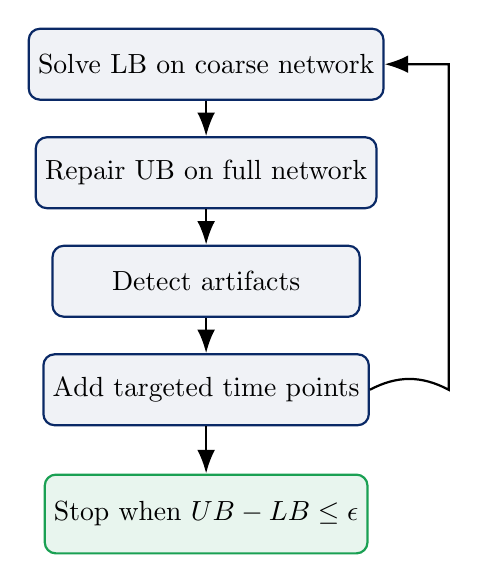
\begin{tikzpicture}[node distance=0.45cm]
    \node[draw=TongjiBlue,rounded corners,thick,fill=TongjiBlue!6,minimum width=3.9cm,minimum height=0.9cm,align=center] (a1) {Solve LB on coarse network};
    \node[draw=TongjiBlue,rounded corners,thick,fill=TongjiBlue!6,below=of a1,minimum width=3.9cm,minimum height=0.9cm,align=center] (a2) {Repair UB on full network};
    \node[draw=TongjiBlue,rounded corners,thick,fill=TongjiBlue!6,below=of a2,minimum width=3.9cm,minimum height=0.9cm,align=center] (a3) {Detect artifacts};
    \node[draw=TongjiBlue,rounded corners,thick,fill=TongjiBlue!6,below=of a3,minimum width=3.9cm,minimum height=0.9cm,align=center] (a4) {Add targeted time points};
    \node[draw=GoodGreen,rounded corners,thick,fill=GoodGreen!10,below=0.6cm of a4,minimum width=3.9cm,minimum height=1cm,align=center] (a5) {Stop when $UB-LB\leq \smallValue$};
    \draw[-{Latex[length=3mm]},thick] (a1) -- (a2);
    \draw[-{Latex[length=3mm]},thick] (a2) -- (a3);
    \draw[-{Latex[length=3mm]},thick] (a3) -- (a4);
    \draw[-{Latex[length=3mm]},thick,bend left=28] (a4.east) to ++(1.0,0) |- (a1.east);
    \draw[-{Latex[length=3mm]},thick] (a4) -- (a5);
\end{tikzpicture}
\end{center}
\end{columns}
\end{frame}

% -------------------- Results --------------------
\begin{frame}{6. 结果：在真实航空实例上显著优于直接求解}
\begin{columns}[T,totalwidth=\textwidth]
\column{0.44\textwidth}
\begin{block}{Base case: Frontier F9}
\centering
\small
\begin{tabular}{lcc}
\toprule
方法 & Raw Model & IA-DR \\
\midrule
UB & -176{,}824.17 & -176{,}843.71 \\
LB & -185{,}214.71 & -176{,}843.71 \\
Gap & 4.75\% & \textbf{0.00\%} \\
时间(h) & 12.00$^*$ & \textbf{10.92} \\
\bottomrule
\end{tabular}
\vspace{0.08cm}

\footnotesize $^*$ 到 12 小时上限仍未收敛。
\end{block}

\vspace{0.1cm}
\small
\begin{itemize}
    \item 最优解激活 \hl{348} 个航班；
    \item 382 个市场中只服务最有利可图的 \hl{120} 个；
    \item \hl{112} 条中转 itinerary vs. 64 条直接 itinerary。
\end{itemize}

\column{0.54\textwidth}
\begin{center}
    \includegraphics[width=0.96\linewidth]{../figure/img/unexpl_raw_end_both.pdf}
\end{center}
\vspace{-0.1cm}
\centering\scriptsize
branch-and-bound 树对比：直接模型不断膨胀，而 IA-DR 很早收敛。
\end{columns}
\end{frame}

% -------------------- Conclusion + future --------------------
\begin{frame}{7. 结论与未来方向}
\begin{columns}[T,totalwidth=\textwidth]
\column{0.53\textwidth}
\begin{block}{结论}
\begin{itemize}
    \item 本文研究的是 \hl{考虑乘客选择的服务网络设计}；
    \item 我提出了 \hl{IA-DR}：行程聚合 + 上界修复 + 动态细化；
    \item 关键价值在于：\hl{既压缩 itinerary 空间，又保留 exactness}；
    \item 在真实大规模实例上，证明了比直接求解更有效且可达到 \hl{0\% gap}。
\end{itemize}
\end{block}

\column{0.43\textwidth}
\begin{block}{未来方向}
\begin{itemize}
    \item 扩展到城际铁路、公交等其他客运网络；
    \item 做更大网络、更多资源类型、multi-day planning；
    \item 融入 crew scheduling、maintenance 等下游约束；
    \item 探索更丰富的 choice model 与 warm start。
\end{itemize}
\end{block}

\vspace{0.2cm}
\begin{center}
\Large \textcolor{TongjiBlue}{\textbf{谢谢！}}
\end{center}
\end{columns}
\end{frame}

% -------------------- Appendix --------------------
\appendix

\begin{frame}{附录 A：基准模型（只列核心结构）}
\small
\begin{block}{SN-PC$(\hat{\discretization})$}
\vspace{-0.25cm}
\begin{align*}
\min\;& \sum_{a\in \full{\flightArc}}\sum_{f\in\fleetSet} \cost_{af}\,\fleetAssignVar_{af}
- \sum_{m\in\marketSet}\sum_{p\in\psgTypeSet}\sum_{r\in\itinInMarket}\sum_{\ell\in\fareClassSet} \demand_{mp}\fare_{r\ell}\shareVar_{rp\ell}\\[0.15cm]
\text{s.t. } & \sum_{a\in \outArcSet{i,t}} \fleetAssignVar_{af} - \sum_{a\in \inArcSet{i,t}} \fleetAssignVar_{af} = 0, \quad \forall (i,t),f \\
& \sum_{a\in \holdingArcTc{\checkTime}} \fleetAssignVar_{af} + \sum_{a\in \flightArcTc{\checkTime}} \fleetAssignVar_{af} \le \fleetAvail_f, \quad \forall f \\
& \sum_{f\in\fleetSet}\sum_{a\in \arcDuringSepTime_{ijt}} \fleetAssignVar_{af} \le 1, \quad \forall (i,j),t \\
& \outAttr_{mp}\shareVar_{rp\ell} \le \attr_{rp\ell}\outsideShareVar_{mp}, \quad \forall m,p,r,\ell \\
& \left(\frac{\adjOutAttr_{mp}}{\outAttr_{mp}}\right) \outsideShareVar_{mp} +
\sum_{r,\ell} \left(\frac{\adjAttr_{rp\ell}}{\attr_{rp\ell}}\right)\shareVar_{rp\ell} = 1, \quad \forall m,p \\
& \sum_{m,p,\ell}\sum_{r\in \itinUsingArc{m}{a}} \demand_{mp}\shareVar_{rp\ell} \le \sum_{f\in\fleetSet}\fleetCap_f\fleetAssignVar_{af}, \quad \forall a\in\full{\flightArc}
\end{align*}
\end{block}
\end{frame}

\begin{frame}{附录 B：算法细节（按模块拆开）}
\small
\begin{columns}[T,totalwidth=\textwidth]
\column{0.33\textwidth}
\begin{block}{LBM}
\begin{itemize}
    \item 在粗时间离散化上建模；
    \item 允许时间弧聚合；
    \item 再对 itinerary 做 path-signature aggregation；
    \item 得到 valid lower bound。
\end{itemize}
\end{block}

\column{0.33\textwidth}
\begin{block}{UBM}
\begin{itemize}
    \item 在 full network 上修复；
    \item 锁定 segment--fleet frequency；
    \item 用 itinerary cuts 抑制收入高估；
    \item 给出 feasible incumbent。
\end{itemize}
\end{block}

\column{0.33\textwidth}
\begin{block}{Refinement}
\begin{itemize}
    \item 检查 chronological violations；
    \item 检查 separation infeasibility；
    \item 检查 phantom revenue；
    \item 针对性加入时间点，继续迭代。
\end{itemize}
\end{block}
\end{columns}

\vspace{0.2cm}
\begin{alertblock}{一句话总结}
\centering
\textbf{用 tighter LB 缩小搜索空间，用 targeted refinement 保证 exactness。}
\end{alertblock}
\end{frame}

\begin{frame}{附录 C：行程聚合为什么能保持下界？}
\begin{columns}[T,totalwidth=\textwidth]
\column{0.42\textwidth}
\begin{block}{直观理解}
\small
\begin{itemize}
    \item 一个 super-itinerary 对应多个原始 itinerary；
    \item 原始 itinerary 之间可能因最小间隔约束而冲突；
    \item 我们不是把 attraction 全部直接相加；
    \item 而是在合法组合上取 \hl{optimistic but valid} 的上界。
\end{itemize}
\end{block}

\vspace{0.12cm}
\begin{equation*}
\attrSuper_{R p\ell} =
\max_{\itinCombSet:\, |\itinCombSet|\le \combLimit_R}
\sum_{\mathscr{O}\in\itinCombSet}\sum_{r\in\mathscr{O}} \attr_{r p\ell}
\end{equation*}

\vspace{0.05cm}
\small
其中 $\combLimit_R$ 由聚合时间窗内可物理共存的服务数量控制。

\column{0.56\textwidth}
\begin{center}
    \includegraphics[width=\linewidth]{../figure/illustrate_valid_combinations/valid_combinations.pdf}
\end{center}
\end{columns}
\end{frame}

\end{document}
